

\documentclass[a4paper, 11pt]{article} 



\usepackage{graphicx} 

\usepackage[parfill]{parskip} % Activate to begin paragraphs with an empty line rather than an indent

%%% PACKAGES
\usepackage{booktabs} % for much better looking tables
\usepackage{array} % for better arrays (eg matrices) in maths
\usepackage{paralist} % very flexible & customisable lists (eg. enumerate/itemize, etc.)
\usepackage{verbatim} % adds environment for commenting out blocks of text & for better verbatim
\usepackage{subfig} % make it possible to include more than one captioned figure/table in a single float
\usepackage{lscape} %turn landscape
\usepackage{amsmath} %math formatting
\usepackage{longtable} % tabular env from markdown
\usepackage[colorlinks, citecolor=blue]{hyperref} % makes for easy anchor tags in document

%formatting allows footnotes to keep black color
\makeatletter
\def\@footnotecolor{red}
\define@key{Hyp}{footnotecolor}{%
	\HyColor@HyperrefColor{#1}\@footnotecolor%
}
\def\@footnotemark{%
	\leavevmode
	\ifhmode\edef\@x@sf{\the\spacefactor}\nobreak\fi
	\stepcounter{Hfootnote}%
	\global\let\Hy@saved@currentHref\@currentHref
	\hyper@makecurrent{Hfootnote}%
	\global\let\Hy@footnote@currentHref\@currentHref
	\global\let\@currentHref\Hy@saved@currentHref
	\hyper@linkstart{footnote}{\Hy@footnote@currentHref}%
	\@makefnmark
	\hyper@linkend
	\ifhmode\spacefactor\@x@sf\fi
	\relax
}%
\makeatother
\hypersetup{footnotecolor=black}

\renewcommand{\thesection}{\Alph{section}.}

\title{EDLD 650: Data Analysis and Replication Exercise (DARE) 4}
\author{David D. Liebowitz}
\date{Due: Feb. 28, 2022} 

\begin{document}
\maketitle



\section{Baseline differences  (3 points)}

\begin{enumerate}
	\item[A1.] In the full ECLS-K data, teachers perceive kindergarten students classified as language learners (ELs) as having substantially lower math and language skills than their peers who also predominantly speak a language other than English at home, but are not classified as ELs. In \autoref{fig:raw}, we present visual evidence of the gap in perceived skills. Numerically, teachers' perceptions of EL-classified students (on a mean zero, standard deviation one scale) is 0.365 \textit{SD} units lower for math and 0.453 \textit{SD} units lower in language. 
	
	These differences should not be interpreted as the causal effect of being classified as EL on teachers perceptions of students' abilities. These differences could be driven by (a) true (potentially observable) ability differences in students who are classified as EL and those who are not; and (b) unobservable characteristics that cause some students to be classified as EL and others not that also drive teacher perceptions.

	\begin{figure}
		\begin{center}
			\subfloat[Math]{
			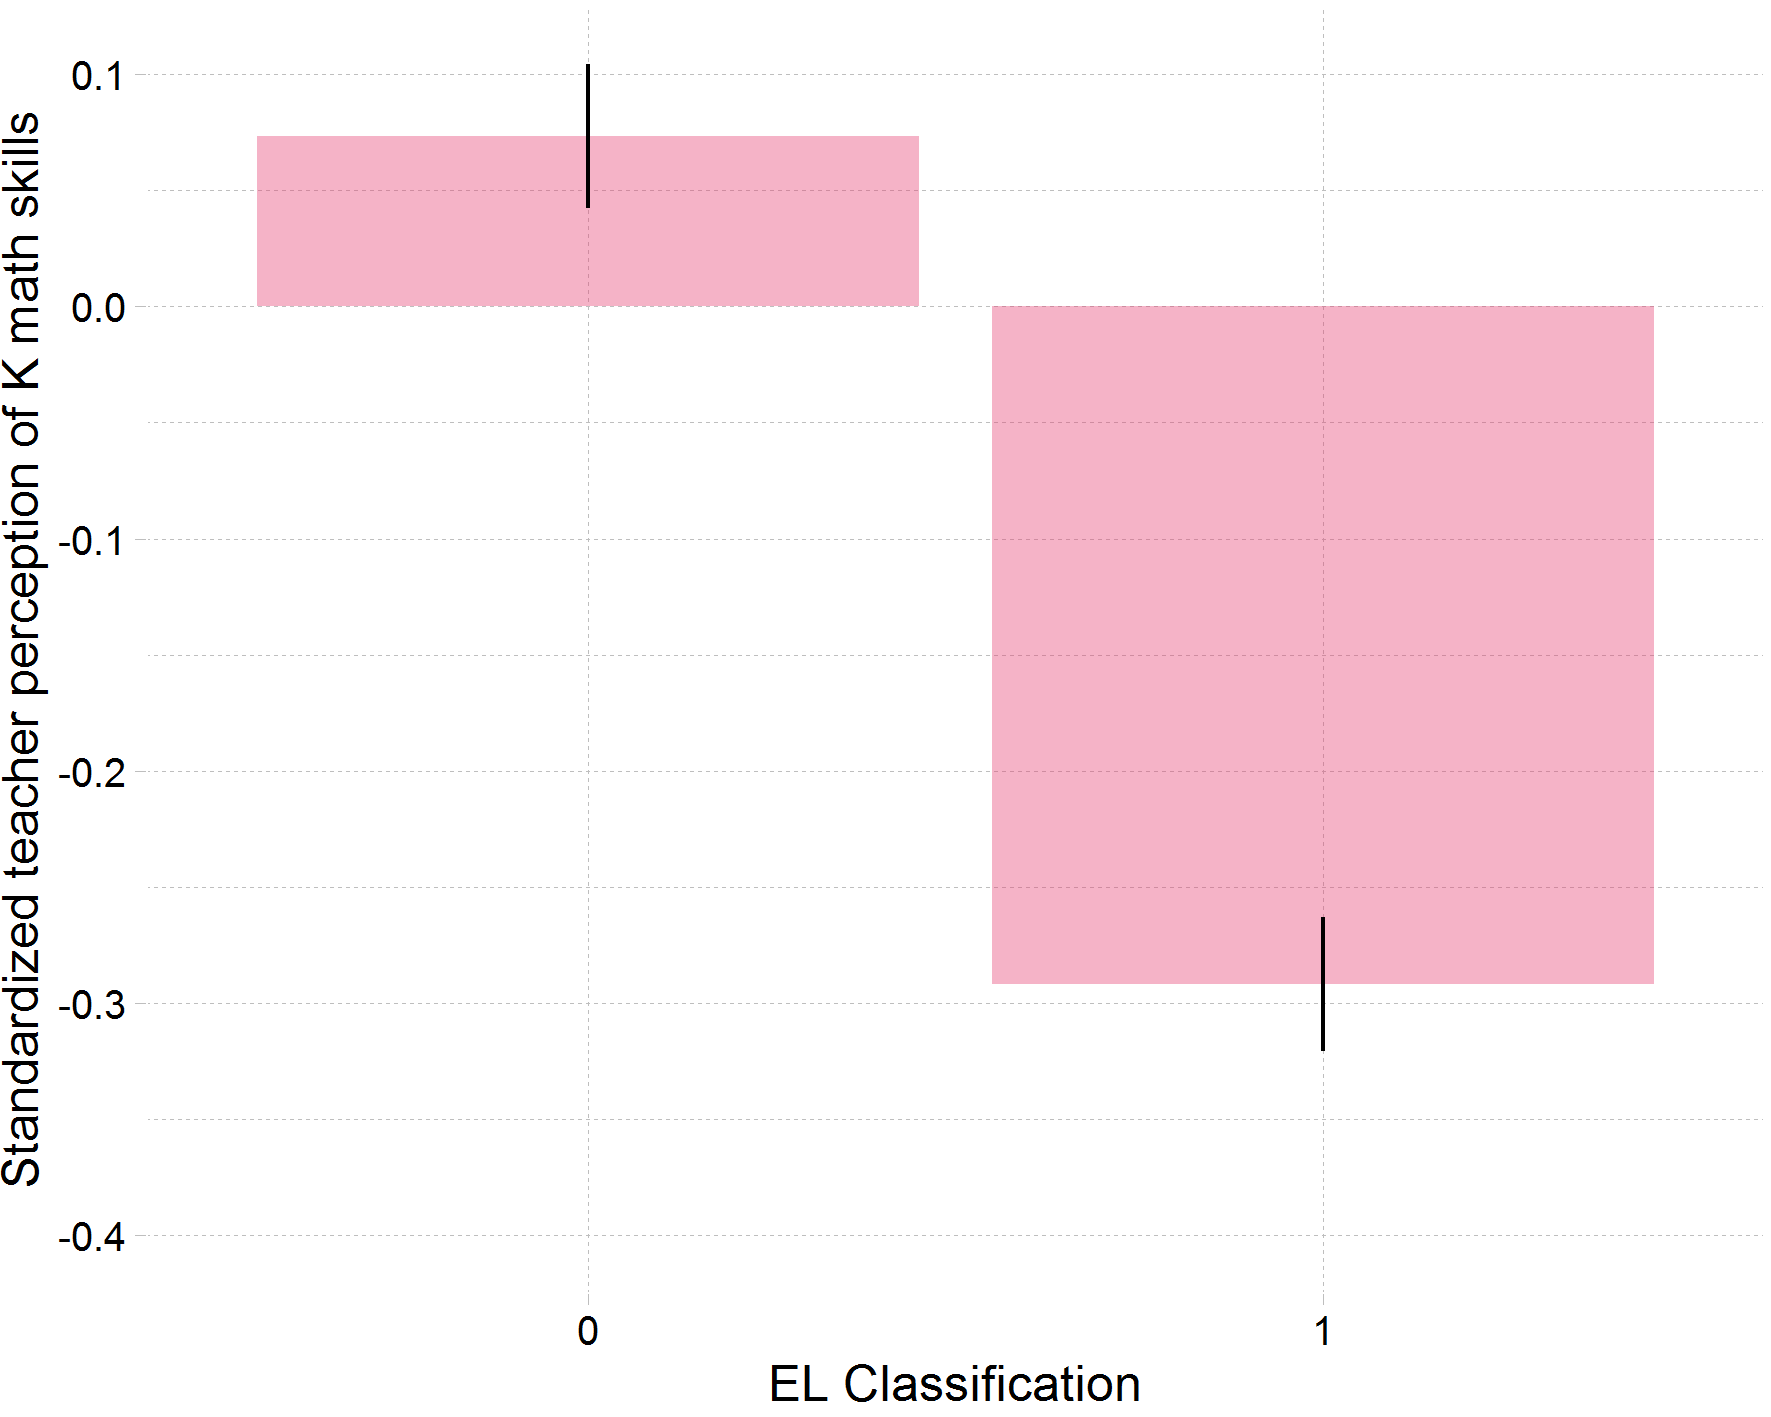
\includegraphics[scale=0.4]{figures/math_percep_raw_diff.png}
		}
			\subfloat[Language]{
			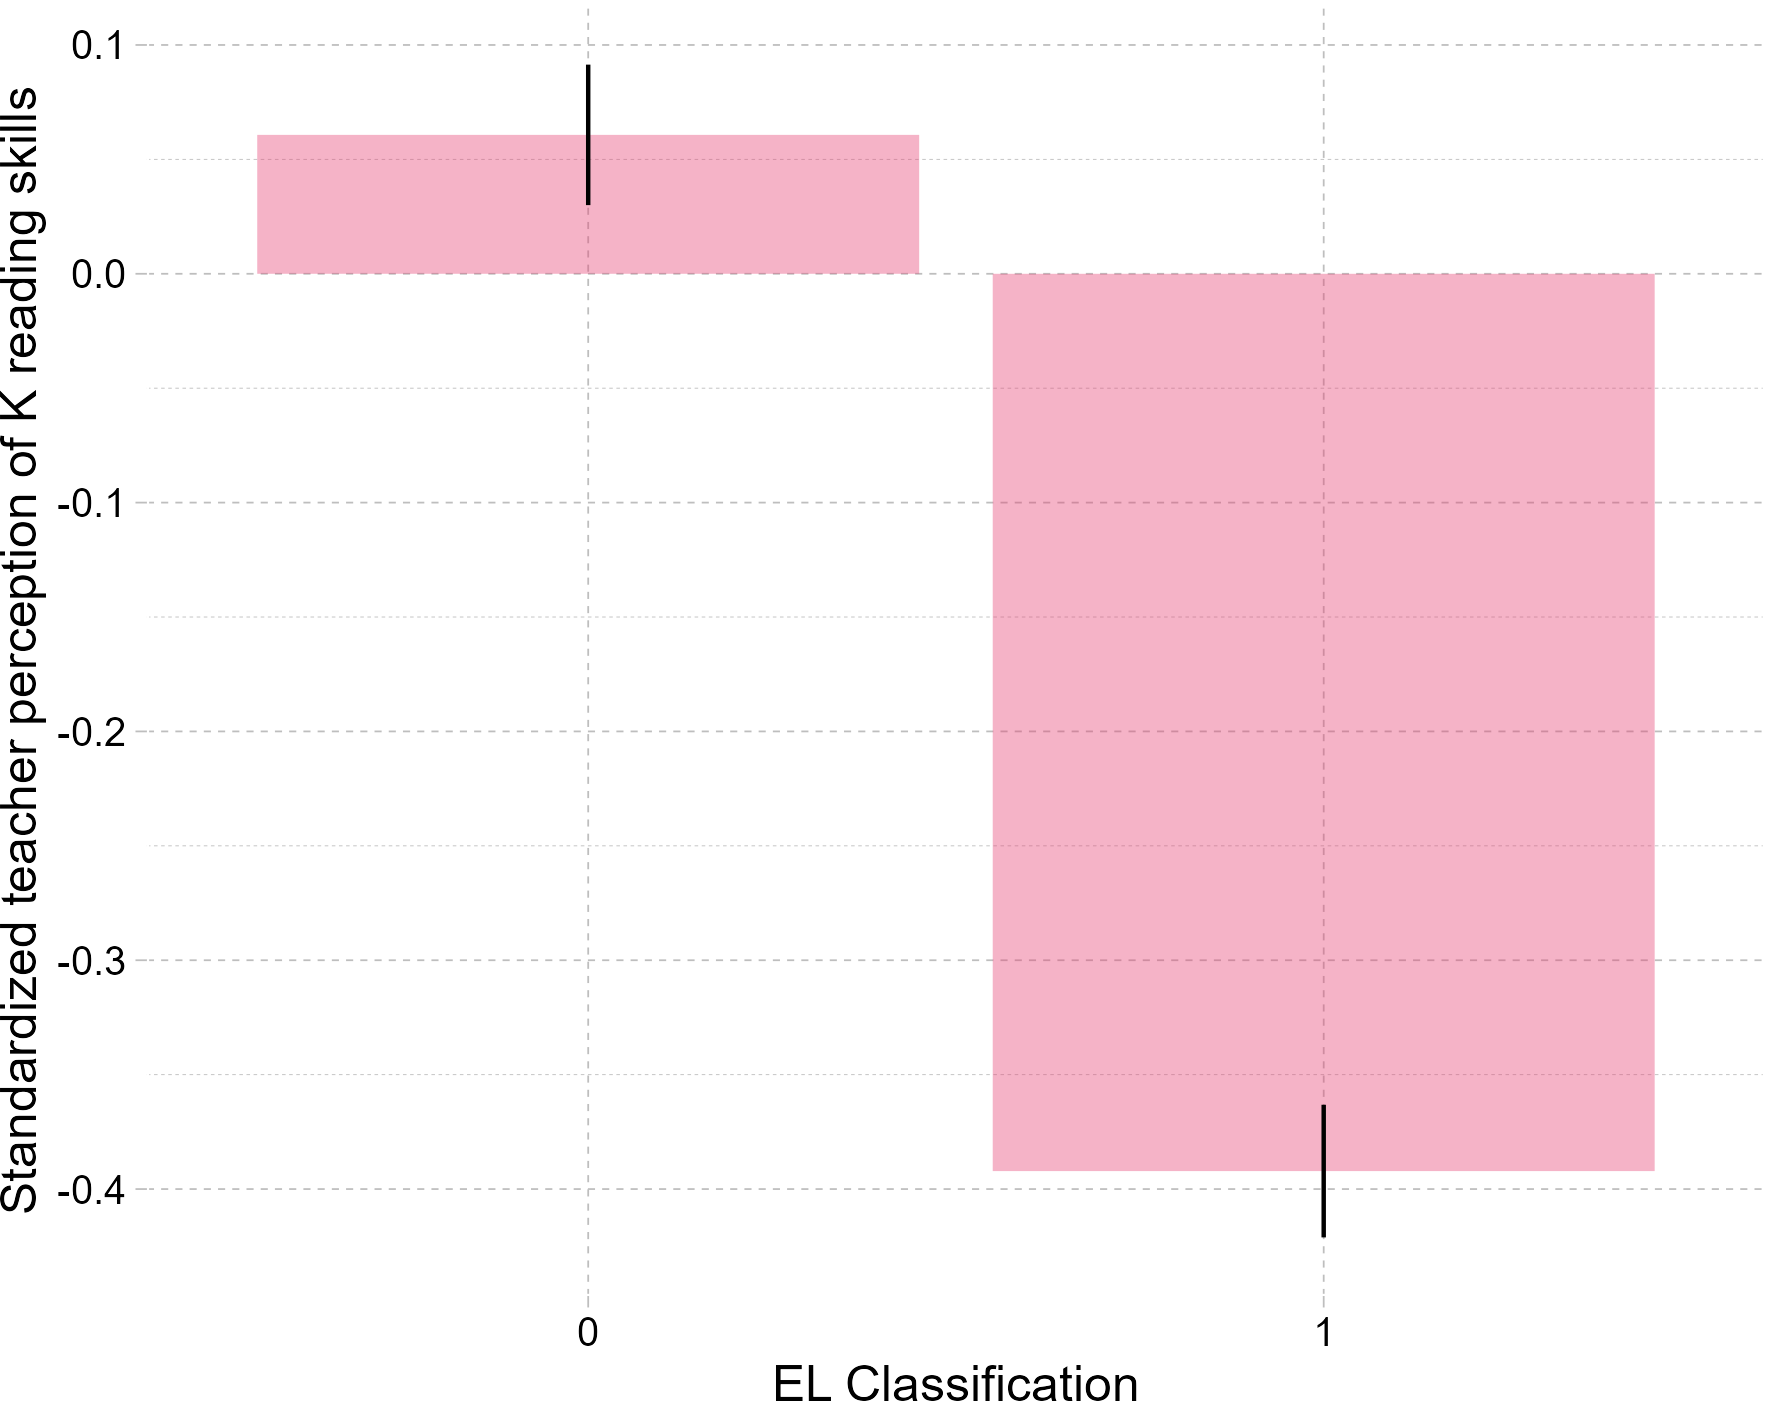
\includegraphics[scale=0.4]{figures/read_percep_raw_diff.png}
			}
			\caption{Standardized teacher perception of math and language skills, by EL program assignment} \label{fig:raw}
		\end{center}
	\end{figure}


	\item[A2.] In fact, as we document in \autoref{tab:descriptives}, students who are and who are not classified as EL are different across many observable dimensions, even though all students in the sample speak a language other than English at home. Specifically, students classified as EL have lower scores on both English language and content tests, are from lower-income families, are less likely to be from rural areas and are more likely to be Hispanic/Latinx than their non-EL-classified peers. The discrepancies in characteristics of individuals in our treatment and control conditions motivate the matching strategies we employ in the subsequent section. 

\begin{table}
	
	\caption{Descriptive statistics by assigned EL status \label{tab:descriptives}}
\centering
\begin{tabular}[t]{lcccc}
	\toprule
	
& Not EL $(N=945)$ & EL $(N=1221)$ & Total $(N=2166)$ & $p$-value \\
\midrule
\textbf{Language Score} & & & & \textless{} 0.001 \\
~~~Mean (SD) & 17.62 (3.32) & 14.55 (4.89) & 15.89 (4.54) & \\
\textbf{Reading Score} & & & & \textless{} 0.001 \\
~~~Mean (SD) & 13.41 (4.57) & 10.79 (4.72) & 11.94 (4.83) & \\
\textbf{K Literacy Score} & & & & \textless{} 0.001 \\
~~~Mean (SD) & -0.49 (0.96) & -1.03 (0.80) & -0.80 (0.91) & \\
\textbf{K Math Score} & & & & \textless{} 0.001 \\
~~~Mean (SD) & -0.50 (1.00) & -1.07 (1.00) & -0.82 (1.04) & \\
\textbf{SES} & & & & \textless{} 0.001 \\
~~~Mean (SD) & -0.21 (0.91) & -0.69 (0.68) & -0.48 (0.82) & \\
\textbf{Female} & & & & 0.396 \\
~~~Mean (SD) & 0.51 (0.50) & 0.49 (0.50) & 0.50 (0.50) & \\
\textbf{Rural school} & & & & \textless{} 0.001 \\
~~~Mean (SD) & 0.14 (0.34) & 0.08 (0.27) & 0.11 (0.31) & \\
\textbf{Hispanic/Latinx} & & & & \textless{} 0.001 \\
~~~Mean (SD) & 0.50 (0.50) & 0.75 (0.44) & 0.64 (0.48) & \\
\bottomrule
\end{tabular}
\end{table}

\end{enumerate}
\pagebreak

\section{Replication and Extension (7 points)}

\begin{enumerate}
	\item[B1.] We begin with a baseline assessment of the probability that a student will be classified as EL, given her observable characteristics. Specifically, we fit the following logistic regression model:

\begin{equation}
	ELPRGRM_{i}= \frac{1}{1+\exp^{\beta_{1}PreLAS_{i} + \beta_{2}EBRS_{i} + \textbf{X}_i\theta_{i} + \epsilon_{i}}}
\end{equation}


	where we estimate the probability that a student will be assigned to an EL program (\textit{ELPRGRM}) as a non-linear function of their language assessment scores (\textit{PreLAS}) and (\textit{EBRS}) which serve as proxies for the district-administered language test used to determine placement. These are our two primary matching variables. We also include a vector of student demographic characteristics (\textbf{X$_{i}$}) that includes their socio-economic status, whether they attend a rural school or not, their gender and their ethnicity (Hispanic/Latinx or not). 

	In \autoref{fig:common}, we plot smoothed densities of students' probability of being classified as EL based on their observable characteristics, based on whether they, in fact, received EL services. While there are broad areas of overlap (often referred to as ``regions of common support''), there are also substantial regions of both high- and low-probability of EL classification where there are large imbalances in the proportion of students by language classification. This further justifies our matching approach.

	\begin{figure}
		\begin{center}
			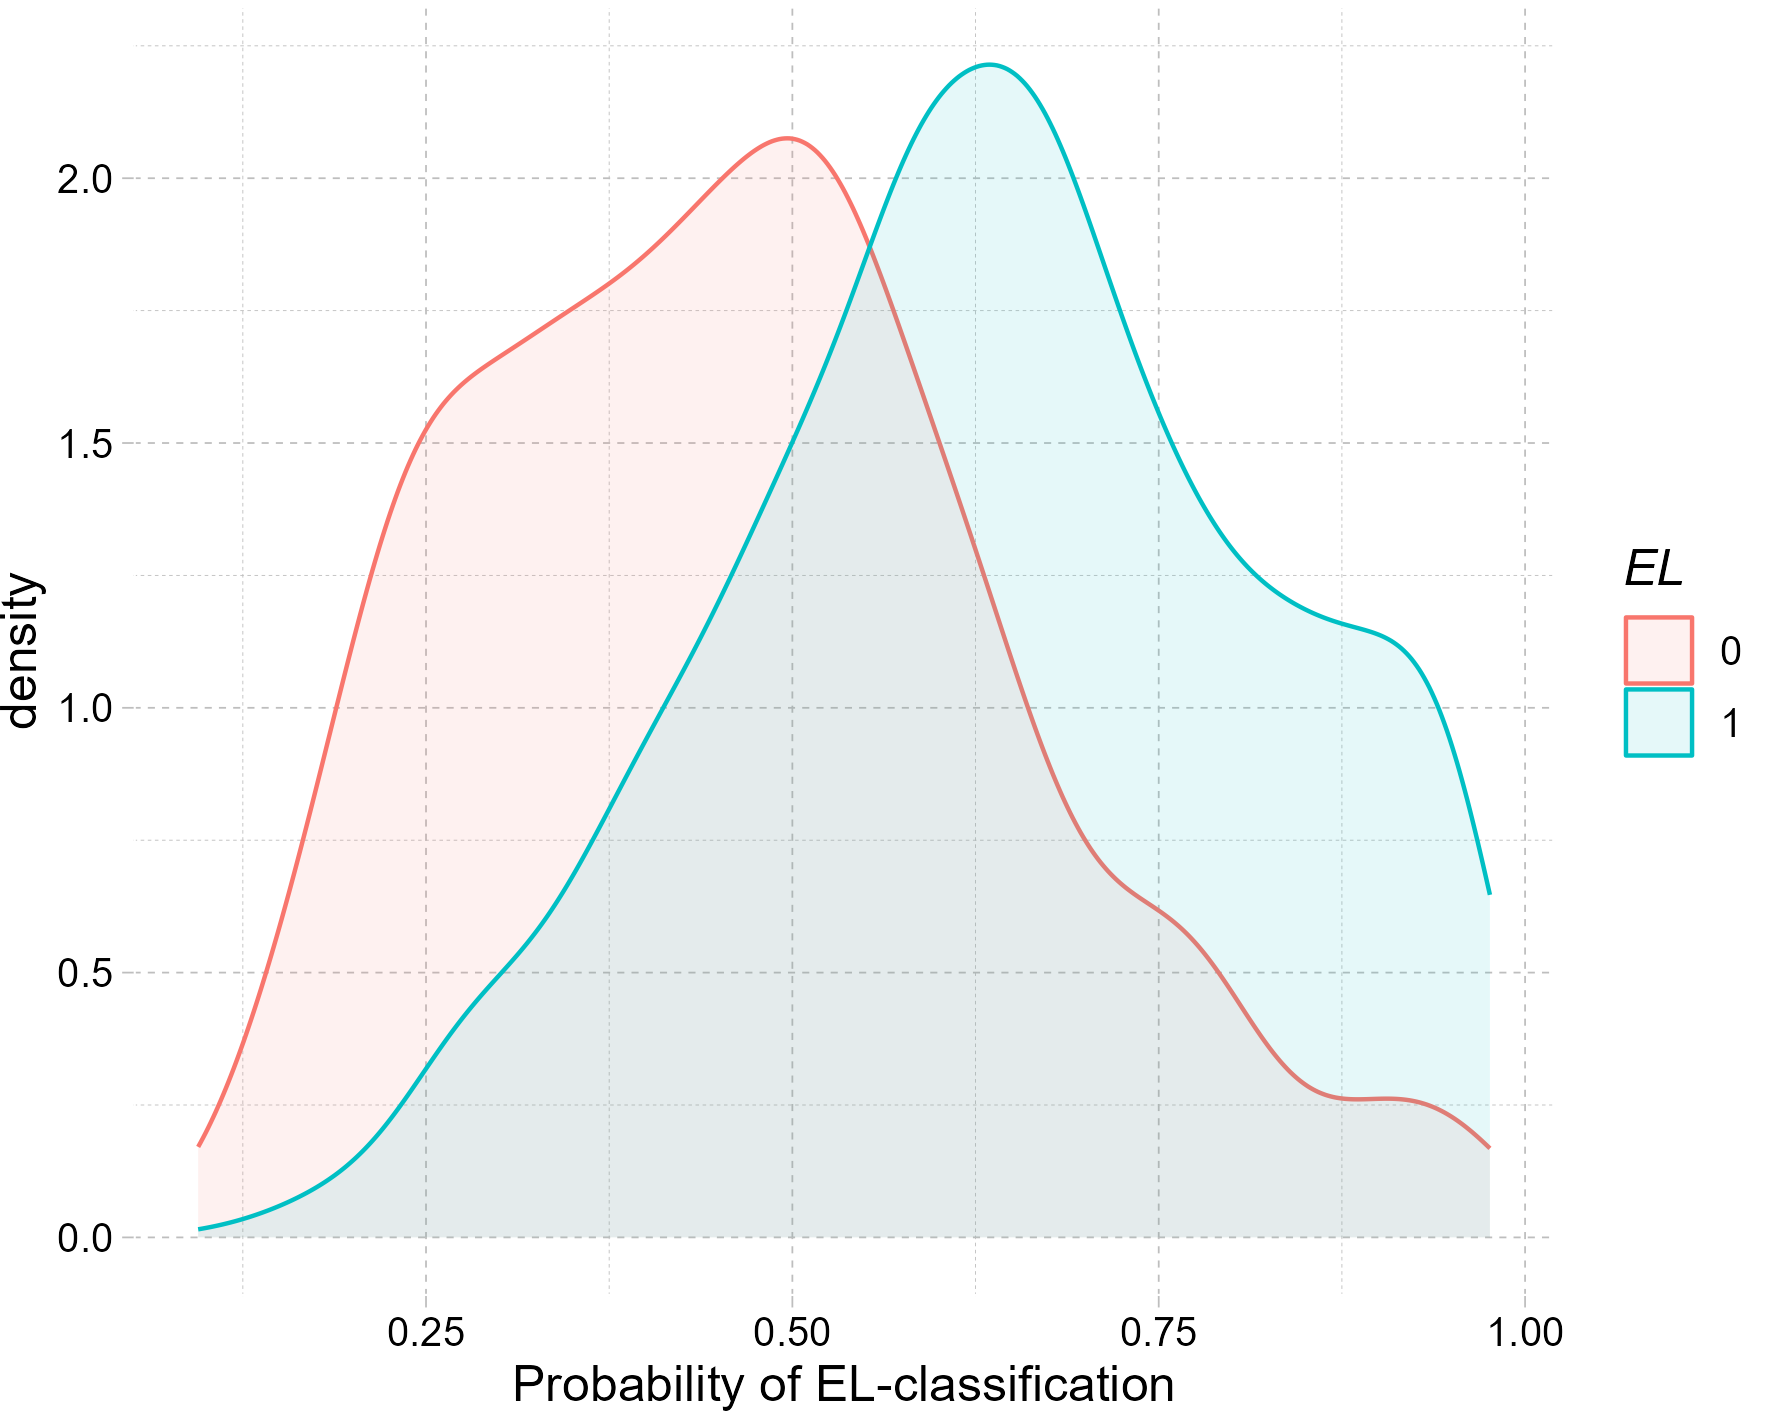
\includegraphics[scale=0.7]{figures/base_common_support.png}
			\caption{Full sample probability of EL program assignment, by actual EL program assignment} \label{fig:common}
		\end{center}
	\end{figure}

	\item[B2.] We implement a Coarsened Exact Matching (CEM) approach in an effort to identify the causal effect of EL-classification on teachers' perceptions of students' abilities. Our primary matching variables emerge from the legal guidelines of the Elementary and Secondary Education Act that dictate that school districts must use students' home language and English proficiency levels to determine their designation as ELs (or not). Specifically, in a sample of students who speak a language other than English at home, we match on a coarsened value of students' Preschool Language Assessment Scale (Pre-LAS) and English Basic Reading Skill (EBRS) assessments. Additionally, we rely on a coarsened version of students' socio-economic status.  For each of these continuous variables, we divide students' scores into quintiles in our sample and match students within quintiles. We also require students to match exactly on gender, attendance in a rural school or not, and Hispanic/Latinx ethnicity (or not). This CEM matching algorithm produces 1627 matched kindergartners, of whom 887 are classified as EL and 740 are not. 
	
	Before proceeding to our estimates of the effects of EL classification, we pause briefly to consider what assumptions must hold in order to interpret our results as supporting causal interpretation. Our central assumption is that, conditional on students' assessed language proficiency, the variation we observe in assignment to treatment (EL) or control (not-EL) conditions depends only on variation in local policy regarding thresholds for EL assignment. Put differently, we assume that students with the same baseline language proficiency and a home language other than English are equal in expectation in their teachers' assessments of their skills, and that no unobservable factors drive categorization of students into either category.
	

	\item[B3.] Our CEM matching strategy substantially reduces the observable differences in the characteristics of EL- and non-EL-classified kindergartners and increases the shared region of common support, but it does not produce perfectly balanced treatment and control samples. In \autoref{tab:cem}, we present descriptive evidence on the 1627-observation matched sample. We achieve perfect matches on all dichotomous variables (\textit{RURAL}, \textit{FEMALE} and \textit{HISPANIC/LATINX}), and we have removed all statistical differences in students' socio-economic status. We have also eliminated all substantive and significant differences in students' English proficiency scores. \autoref{fig:cem_common} provides graphical evidence of the quality of our matches. As compared to \autoref{fig:common}, we see evidence of much greater regions of common support, but remaining differences in the distributions of EL and non-EL students' probability of receiving the treatment.

\begin{table}
	
	\caption{CEM-matched descriptive statistics by assigned EL status \label{tab:cem}}
	\centering
	\begin{tabular}[t]{lcccc}
		\toprule
		

& Not EL $(N=740)$ & EL $(N=887)$ & Total $(N=1627)$ & $p$-value \\
\midrule
\textbf{Language Score} & & & & 0.786 \\
~~~Mean (SD) & 14.97 (5.02) & 14.91 (4.98) & 14.94 (5.00) & \\
\textbf{Reading Score} & & & & 0.909 \\
~~~Mean (SD) & 10.91 (4.89) & 10.89 (4.85) & 10.90 (4.87) & \\
\textbf{SES} & & & & 0.752 \\
~~~Mean (SD) & -0.66 (0.74) & -0.67 (0.72) & -0.67 (0.73) & \\
\textbf{Rural school} & & & & 1.000 \\
~~~Mean (SD) & 0.03 (0.17) & 0.03 (0.17) & 0.03 (0.17) & \\
\textbf{Female} & & & & 1.000 \\
~~~Mean (SD) & 0.47 (0.50) & 0.47 (0.50) & 0.47 (0.50) & \\
\textbf{Hispanic/Latinx} & & & & 1.000 \\
\bottomrule
\end{tabular}
\end{table}	

	\begin{figure}
		\begin{center}
			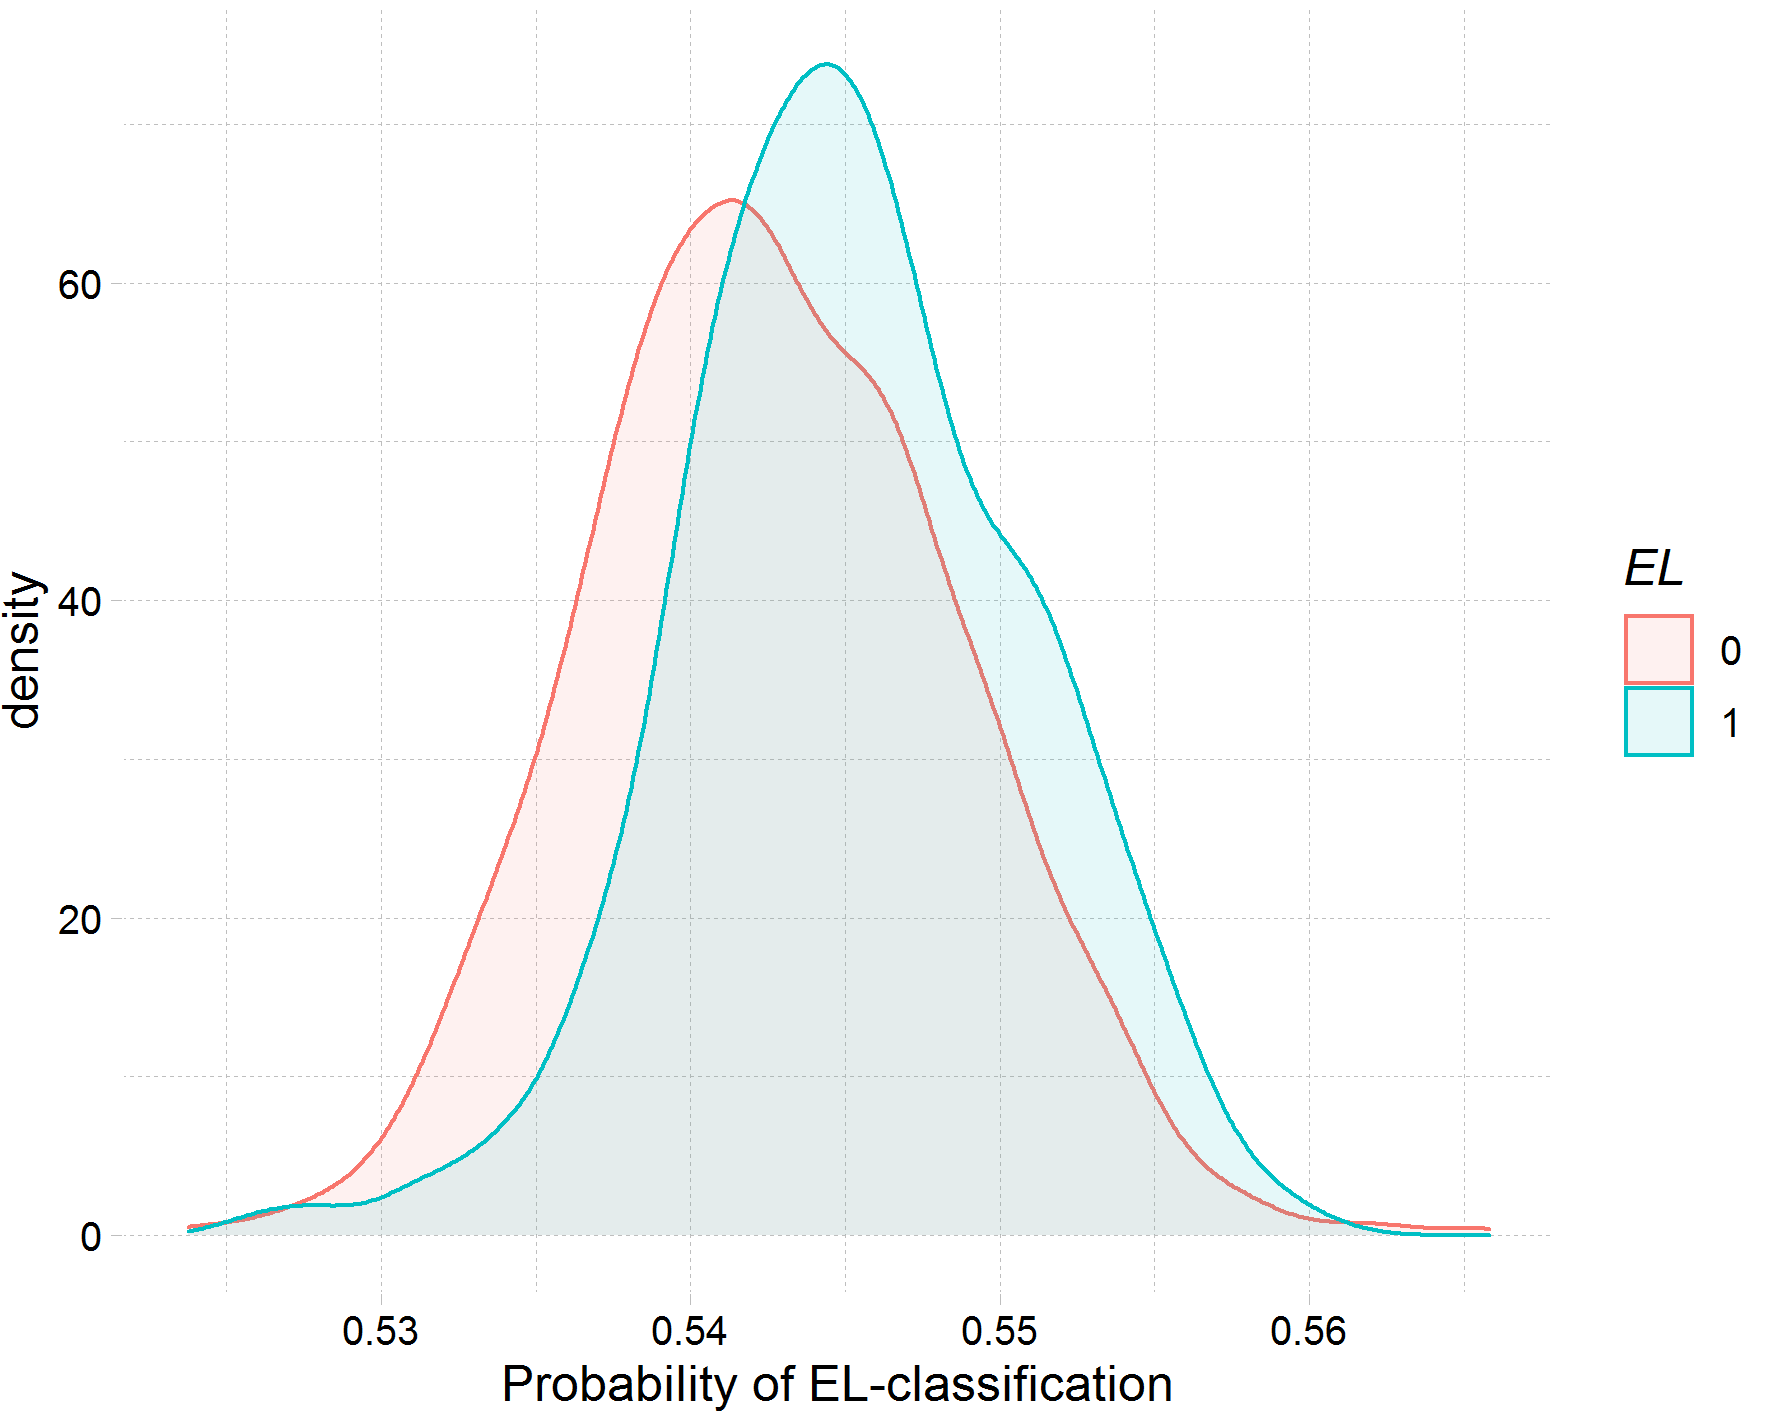
\includegraphics[scale=0.7]{figures/cem1_common_support.png}
			\caption{CEM-matched sample probability of EL program assignment, by actual EL program assignment} \label{fig:cem_common}
		\end{center}
	\end{figure}

	While this matching strategy has served to remove much of the bias introduced by baseline characteristic differences between the two groups, it is not perfect and may merit further reconsideration. Our CEM strategy has common support throughout the distribution, so we are still able to generalize to the same population of students who predominantly speak a language other than English at home. However, our common support is not perfect, and we have reduced our sample substantially. We would likely want to vary the width of the bins on which to match our continuous variables or to include more matching variables that better accounted for differences in students categorized as EL and not. The first strategy is preferable as it preserves the criteria-based assignment we have theorized is driving selection into treatment. This allows us to better defend our identification assumptions. However, we risk losing common support within our strata. The second approach will preserve more of our sample, but we stray further from our hypothesized selection process which threatens the assumptions of our overall approach.

	\item[B4.] As a robustness check, we estimate an alternate Propensity Score Matching (PSM) algorithm in which we match treated (EL) students to their nearest-neighbor by propensity score (with replacement) to construct a separate matched sample. We present analagous evidence in \autoref{tab:psm} on the quality of our matches and \autoref{psm_common} on the region of common support. Our PSM approach produces roughly equal quality matches, with around the same sample size. However, while we fail to reject the null hypothesis, some of our balancing variables are substantively different across students who are and are not classified as EL (in particular their family-income levels, which differ by 7 percentage points). In all cases, we found a match for each of our treated units, and we did so without requiring the sample to become imbalanced because none of the treated units fell outside the region of common support.\footnote{Additionally, we did not specify a caliper-width outside of which we would refuse to allow students to match which would have led us to drop some of the treated units from our sample.}

	\begin{figure}
		\begin{center}
			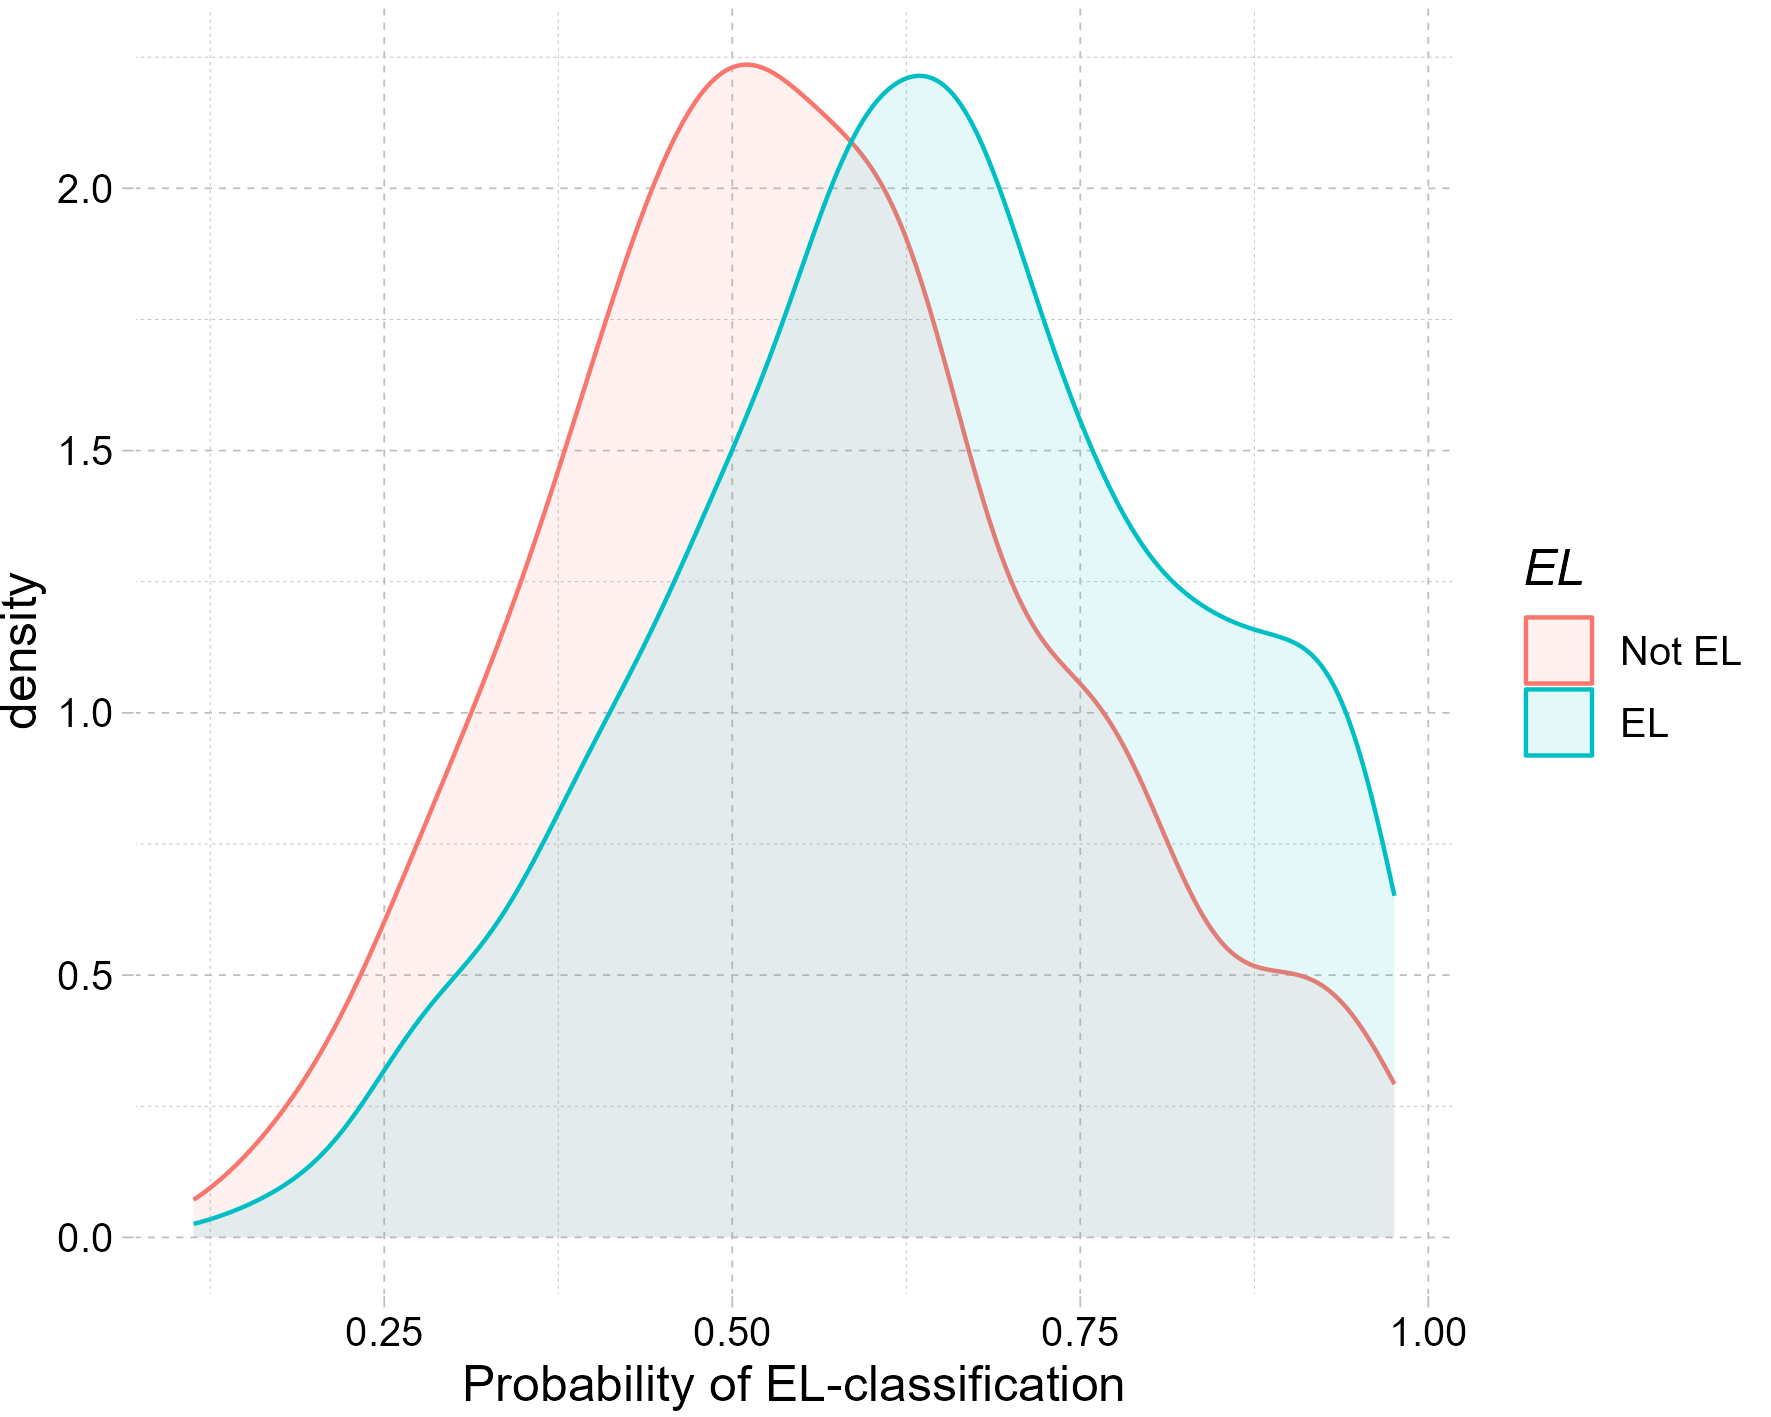
\includegraphics[scale=0.7]{figures/psm_common_support.png}
			\caption{PSM-matched sample probability of EL program assignment, by actual EL program assignment} \label{psm_common}
		\end{center}
	\end{figure}

\begin{table}
	
	\caption{PSM-matched descriptive statistics by assigned EL status \label{tab:psm}}
	\centering
	\begin{tabular}[t]{lcccc}
		\toprule

& Not EL $(N=480)$ & EL $(N=1221)$ & Total $(N=1701)$ & $p$-value \\
\midrule
\textbf{Propensity score} & & & & 0.994 \\
~~~Mean (SD) & 0.64 (0.18) & 0.64 (0.18) & 0.64 (0.18) & \\
\textbf{Language Score} & & & & 0.488 \\
~~~Mean (SD) & 14.90 (4.98) & 14.55 (4.89) & 14.65 (4.92) & \\
\textbf{Reading Score} & & & & 0.261 \\
~~~Mean (SD) & 10.79 (4.79) & 10.79 (4.72) & 10.79 (4.74) & \\
\textbf{SES} & & & & 0.560 \\
~~~Mean (SD) & -0.76 (0.66) & -0.69 (0.68) & -0.71 (0.68) & \\
\textbf{Rural school} & & & & 0.153 \\
~~~Mean (SD) & 0.06 (0.23) & 0.08 (0.27) & 0.07 (0.26) & \\
\textbf{Female} & & & & 0.608 \\
~~~Mean (SD) & 0.47 (0.50) & 0.49 (0.50) & 0.48 (0.50) & \\
\textbf{Hispanic/Latinx} & & & & 0.890 \\
~~~Mean (SD) & 0.77 (0.42) & 0.75 (0.44) & 0.75 (0.43) & \\
\bottomrule
\end{tabular}
\end{table}


	\item[B5.] In \autoref{tab:match}, we present results from OLS, CEM and PSM estimates of the effects of EL-classification on teacher perceptions of student abilities in math and reading in kindergarten. Models 1 and 5 estimate the simple bivariate relationship and are equivalent to the mean differences we present in A1. In Models 2 and 6, we introduce a vector of language proficiency and student background covariate adjustments. These are the typical way that analysts attempt to account for bias in multiple regression methods. These result in a substantial attenuation of the relationship between EL-classification and teacher perceptions; though both relationships remain relatively large in magnitude and significant. Models 3 and 7 present our estimates of the relationship in our CEM-matched sample. The coefficients imply that an EL classification reduces teachers' perception of student ability in math by around one-twentieth of a standard deviation (though imprecisely estimated) and an imprecisely estimated null effect in reading. Finally, we present the results of our estimates in the PSM-matched sample in Models 4 and 8. Our estimate of the effect of classification on math and reading are slightly negative, but in both cases statistically equivalent to zero.

	\item[B6.] We use a set of matching approaches to estimate the potentially causal effect of EL-classification on teachers' perceptions of kindergarten students' math and language abilities. We find that traditional statistical methods to adjust for background characteristics would misrepresent the effect of EL classification on teachers' perceptions of students' abilities. Whereas covariate-adjustment approaches would characterize EL classification as resulting in reduced teacher perceptions' of students' ability by 0.16 to 0.18 \textit{SD}, matching approaches suggest that such classification does not change teacher perceptions for students in Kindergarten. Our preferred specification uses coarsened exact matching to identify a group of non-EL classified students who are equal in expectation to the EL-classified group. In these estimates, we cannot rule out that the effects of EL classification are indistinguishable from zero for teachers' perceptions of students' math and reading abilities. We argue our estimates should be understood as causal effects of EL classification if our assumption that students with the same language proficiency score are classified differently only based on idiosyncrasies of local policy. 
	
\end{enumerate}

\begin{landscape}

% Table created by stargazer v.5.2.3 by Marek Hlavac, Social Policy Institute. E-mail: marek.hlavac at gmail.com
% Date and time: Fri, Mar 01, 2024 - 3:55:14 PM
\begin{table}[!htbp] \centering 
  \caption{Comparison of estimates of EL classification on teacher perceptions} 
	\label{tab:match}  
\begin{tabular}{@{\extracolsep{5pt}}lcccccccc} 
\\[-1.8ex]\hline 
\hline \\[-1.8ex] 
 & \multicolumn{8}{c}{\textit{Dependent variable:}} \\ 
\cline{2-9} 
\\[-1.8ex] & \multicolumn{4}{c}{Teacher Math Perception} & \multicolumn{4}{c}{Teacher Language Perception} \\ 
 & OLS & OLS & CEM & PSM & OLS & OLS & CEM & PSM \\ 
\\[-1.8ex] & (1) & (2) & (3) & (4) & (5) & (6) & (7) & (8)\\ 
\hline \\[-1.8ex] 
 EL-classified & $-$0.365$^{***}$ & $-$0.160$^{***}$ & 0.004 & $-$0.035 & $-$0.453$^{***}$ & $-$0.188$^{***}$ & $-$0.064 & $-$0.022 \\ 
  & (0.043) & (0.043) & (0.046) & (0.051) & (0.043) & (0.039) & (0.043) & (0.047) \\ 
  & & & & & & & & \\ 
\hline \\[-1.8ex] 
Student Chars & No & Yes & Yes & Yes & No & Yes & Yes & Yes \\ 
Observations & 2,166 & 2,166 & 1,627 & 1,701 & 2,166 & 2,166 & 1,627 & 1,701 \\ 
R$^{2}$ & 0.033 & 0.194 & 0.165 & 0.175 & 0.050 & 0.321 & 0.281 & 0.291 \\ 
\hline 
\hline \\[-1.8ex] 
\multicolumn{9}{l}\textit{Notes:} {$^{*}$p$<$0.05; $^{**}$p$<$0.01; $^{***}$p$<$0.001. Table presents coefficients and standard errors (in parentheses).} \\ 
\end{tabular} 
\end{table} 

\end{landscape}




\end{document}
